\documentclass{article}
\usepackage[utf8]{inputenc}

\title{Design Document - Software Desing}
\author{Joni, Johanna, Max, Viktor}
\date{2021}


\usepackage{graphicx}


\begin{document}

\maketitle

\tableofcontents

\newpage

\section{Used Terms}

\emph{Project} = Project encompassing Application, Documentation and Unit Tests
\emph{Application} = Gui Application developed based on course requirements


\section{Design Philosophy And Development Methodology} % JOHANNA

The design process of the \emph{Application} has been based on agile development process. As a team we recognized that old, dusty and tried but not so true waterfall way of doing software development where first you design,  then you implement and lastly double the time used in design step to correct the initial design to match reality made no sense to us. Luckily now days it also doesn't makes sense most professional software developers and agile methods are exceedingly common in software development. So in beginning of the project we decided to create a clear concept of software structure and usable UI design based on the requirements of user interaction with the software. Structure was not defined in function level or even in class level but as imaginary modules that we could justify based on the requirements. These modules can and should be split to classes and class methods when actually developing the functionality but this way the realities that surround said element can be taken in to consideration at the time of its design. To coordinate working and identify that time for more detailed design of a module has arrived it is essential that communication between development team is active and timely. As a way of having accurate collective understanding of state of the development our team has had remote meetings once or twice a week. Task oriented workflow has also been very useful tool for discovering the need for collaborative design in the software. For tracking and distributing tasks we have used online kanban board. 

Another possible down fall of agile development is that in worst case the documentation of finished software is sub-par or non-existent. To solve the issue of having accurate documentation of the \emph{Application} our project uses Doxygen to generate up to date and nice to look at documentation of the source code in the level of detail we could only dream of if creating the documentation by hand and/or before the source exists.


\section{Emerging Design Patterns}	% JONI

Desing of the program follow Model Controller View paradigm. All data is deployed
to QML engine via a model that is only responsible for modeling 2d x-y diagram.
Modifying data in model is done via Ui Controller and data is displayed via QML
Element acting as view. These desing steps are meant to keep the responsibilities of
different classes as clear and simple as possible. Also interface between model and
view is very simple to use from c++ as model is read to QML view automatically.

Class structure tries to be as simple as possible. In other words this is called Single
responsibility principle. Class diagram is very streamlined and classes have no
redundant connections between them. Alltough even while keeping amount of classes
to minimum, each class is clearly responsible for a minimal amount of tasks.

Open-closed principle is being used in the design. Program is designed so it can be
extended easily and does not need to modify already existing code. Also it makes
extensions more reliable and possible coming bugs from the extension will be
minimized. Class structure also allows adding additional apis quite easily as each api
is abstracted as a C++ class.

Project follows also resource acquisition is initialization. Every classes resource
allocation is made during object creation by constructor and resource deallocation is
done during object destruction. This mean there will be no resource leaks and every
object will have resources only when alive.


\newpage

\section{High Level Description of \emph{Application}} %VIKTOR

The \emph{Application} is a Qt/Qml computer program targeting Windows 10 environment. \emph{Applications} core functionality consists of fetching data from online APIs and displaying that data as different style graphs. Inner workings of the \emph{Application} is depicted in Figure 1.


\begin{figure}[htbp]
\centering
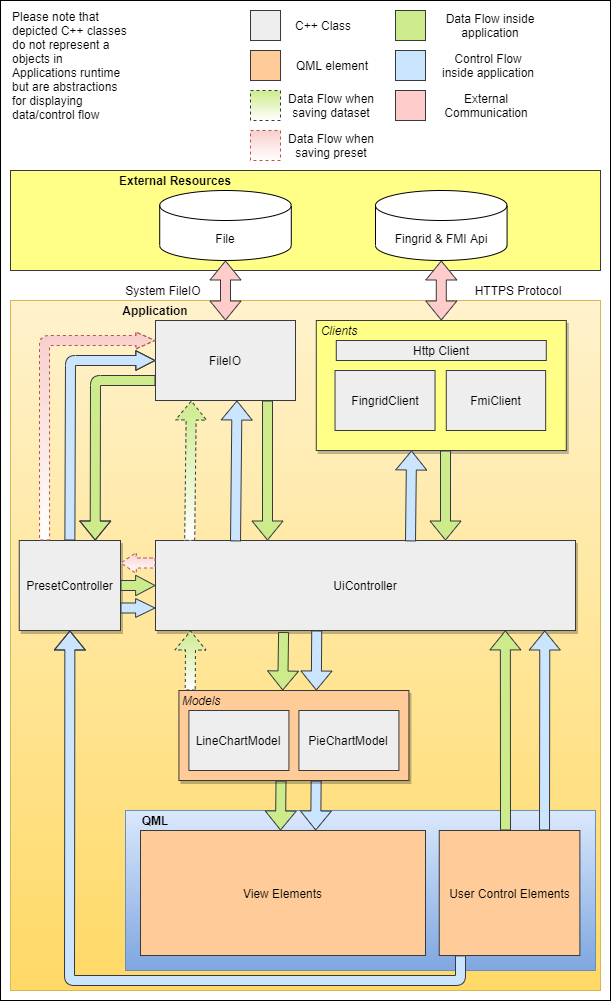
\includegraphics[width=0.52\textwidth]{classdiagram}
\caption{ Class diagram of the \emph{Application} with data and control flow}
\end{figure}


\pagebreak

\emph{Application} follows a \emph{model}, \emph{view} and \emph{controller} design paradigm. This is accomplished by having \emph{controller} classes for monitoring user inputs and conveying user specified data from client classes to \emph{model} classes, \emph{model} classes with user friendly abstraction of the state of \emph{view} element and \emph{view} elements that  can display the abstraction created by \emph{model} class as GUI element. From Figure1 one can see that control and dataflow in \emph{mvc} classes form a clear one way loop. In this loop user interacting with \emph{User Control Elements} causes \emph{UiController} to receive method calls and element state data from GUI and convey data based on those to models. When internal state in model is matching of that specified by user via GUI, controller class tells model to publish its internal state to view element. Model then transfers its internal state to \emph{View Elements} which display the data in model as GUI graph.  It is also good to notice that models used in application cannot be modified trough GUI so there is no reason for data flow out of the models. From with in the \emph{mvc} loop another clear loop emerges. Second loop consists of transactions between controller classes and different clients that fetch data to be used in \emph{mvc} loop from different sources. Here control and data flow is bidirectional instead of \emph{mvc} loops unidirectional flow as data is requested via method calls and delivered via return values.

In Addition to basic data that is fetched from the external resources, there is also some static utility data models which are created by controller classes and used in Qml. These include things like list with all month names. As Qt Framework makes creation of these models easy and they are static, they were excluded from Figure 1. 

Saving data sets is implemented as functionality of \emph{LineChartModel}, \emph{UIController} and \emph{FileIO}. \emph{UIController} implements a methods for saving and loading currently displayed datasets. When data set is saved \emph{UIController} gets the currently displayer \emph{LineChartGraph} structure from its model and passes it along side with the dataset name to \emph{FileIO}. When saving data set \emph{FileIO} converts the \emph{LineChartGraph} in to JSON document and writes it to a file. When loadig a preset FileIO reads previously saved data set from file and parses it in to a \emph{LineChartGraph} which is returned to \emph{UIController} that passes it along to its \emph{LineChartModel} and publishes the model. \emph{UIController} provides also a model of all saved data set names, which is used in UI for selecting what data set to load. When new data set is saved, its name is added to this model. Currently saving a data set is not supported for pie charts.

Besides the fetching, displaying and saving data outlined before, the \emph{Application} has also preset saving feature. This feature allows user to save current user iterface sate in to a file and to load saved user interface from file. This is achieved via \emph{PresetController} class. \emph{PresetController} is a friend class of \emph{UIController} so there is no need for public interface in \emph{UIController}. \emph{PresetController}  is published to QML Context in same manner as \emph{UIController} and it implements invokable interface for saving and loading presets as well as a model of saved preset names. When preset is saved by calling the save function \emph{PresetController} reads the state of interface state variables in UIControllers in to structure and passes it alongside with the name to \emph{FileIO} Class which creates a JSON document out of the preset and writes it in to a file. After saving a preset its name is updated in to the model with saved data set names and it can be loaded by calling the load preset function. When preset is loaded, its name is passed to \emph{FileIO} class which reads the saved JSON document and parses the contents in to preset structure which is returned to \emph{PresetController} which sets the internal state of \emph{UIController} in to corresponding state and does a search.

Data that is moved inside the is typed as abstractions which are designed to work with models. For example when data intended to be displayed as line graphs e.g. using the \emph{LineChartModel}, it is typed as \emph{LineChartGraph}, which is a abstraction of 2d  graph that holds line charts and other attributes like name of the graph. Lines are stored and passed around as \emph{LineCharts} which is a abstarction for line chart and implements some utility methods for line data like min and max values for each axis.  Client classes are responsible for parsing data acquired from online APIs to \emph{LineChartGraphs} so there is no need for altering the data after it is parsed in the client classes.


\newpage



\section{Third Party Technology}	%MAX

The \emph{Project} contains three third party libraries. Firstly the Project is a Qt project so Qt 5.14 framework and its QML capabilities are used heavily to build the back end and GUI. Reason for selecting Qt as the framework for the project was that it is world leading C++ GUI framework and only common programming language suitable for GUI development that our team knew was C++.  Second third party library used is Google Test unit testing framework. This is used in the unit test project to make writing unit tests more convenient. Google Test was selected as some of the team was familiar with it.  Last third party techonology used is 'xml2json' header only library that converts XML documents to JSON documents. Need for this library arouse from the fact that Fmi OpenAPI does not provide its data in JSON form as Fingrid API does. Third party converter was introduced to the project to enable all data fetched from APIs to be parsed using same tools. This helped create synergy between developers developing the client classes as problems that arose from underlying data format were common between different APIs.


\section{Self Evaluation}	%MAX

Adopting agile methods instead of traditional design processes turned out to be an excellent choice for the software development process. Needed modules and interaction between them changed throughout the development process so it was beneficial that there was no rigid design plan that would have needed to be continuously altered. As is typical in modern software development all the user requirements were not known in the beginning of the development process which further made agile methods suitable. Meeting remotely once in a week and trying to divide development into tasks which could be completed in about a week ensured that there was continuous progress going on and if problems were noticed they could be discussed and solved together as a team.

The implementation of our application is following the design almost exactly as planned. Obviously there has been minor modifications to class specific matters such as the user's choice of date was done by storing one calendar widget's date (start date) to a variable. It was designed with the idea that data from histroy could be only a day long. It made more sense to store the user's chosen date from two different calendar widgets to two different variables since there was subsequently added requirement that the application must show data from long periods of time meaning the application also needed a chosen end date. 
Also we found out that instead of storing data from API's to structs within API-client classes, storing their parsed data to LineChart class in form of a struct holding vector of LineCharts depending on the UIControllers search case makes it easier and more clear to implement the rest of the application. 

We also came to the conclusion that some designs for the future implementation should be changed. There was originally only one class designed for saving data into a file. At some point we thought that it would be better if there were also another class for controlling the saved data.
Our original design was done in mind that one UIController class would control the charts view and the saved data view. The design was modified so in the future we will have own controllers for both of the views. This was scrapped later on when we figured out that it wouldn't make sense to even make another view for saved datasets since the whole view would've been very bare. Since we ended up with only one main view we stuck with the idea of using only one controller.

As the application was reaching its final form and even though agile methods were present in our software development, it’s safe to say that some modifications were made to the previous design. We originally had designed a wrapper class that would call FileIO from UIController. We hadn’t designed it too thoroughly at that point and as we went on with the implementation, we realized that there is no need for such class. UIController can call FileIO directly and the wrapper class wouldn’t have had any purpose. 
Another major change was that originally, we used to handle the graphs as singular graphs. as we were reaching towards the end, it made more sense to change things a bit and handle the graphs as a group of graphs. Meaning we would store all the information gathered from the API call to one data structure, instead of multiple different ones that would then be given to a graph.

Previously mentioned things weren’t necessary to implement all the features we’ve implemented. They were changed for the sake of making things clearer and following good software development practices. Considering that our design got more detailed as the application was getting towards the end, no major changed were needed to make during the process.

The software was tested twice during the process. First testing was executed when most of the requirements were implemented and second when the software was finished but early enough to make possible fixes before required releasing date. The most severe finding during the first testing was that software crashes with incorrect query settings, like giving invalid location or setting start date after end date in time range. It was also noticed that in a certain query the software crashes with longer time range (6 months). There were also some graphs with incorrect or no name, text that was too long to be displayed properly and slightly different layout configurations in different search views. During the second testing it was found that in a certain error situation the software did not indicate that any error had happened, as well as a couple of smaller inconveniences. Noticing and fixing these bugs before releasing was essential.




\end{document}
